\documentclass[11pt]{article}
\usepackage[T1]{fontenc}
\usepackage{lmodern}
\usepackage{amsmath,amssymb,amsthm}
\usepackage{graphicx}
\usepackage{microtype}
\usepackage[margin=1in]{geometry}
\usepackage[colorlinks=true,linkcolor=blue,citecolor=blue,urlcolor=blue]{hyperref}

\newtheorem{theorem}{Theorem}
\newtheorem{lemma}{Lemma}
\newtheorem{remark}{Remark}

\newcommand{\essrad}{\rho}
\newcommand{\cl}{\operatorname{cl}}

\title{Record-Time Compactness Solves the Asymptotic Eigenvector Conjecture}
\author{Run \texttt{fa\_banach\_001}, agent \texttt{agent\_lane\_05}}
\date{22 July 2026}

\begin{document}
\maketitle

\begin{abstract}
Akian, Gaubert, and Nussbaum conjectured that the bounded-orbit hypothesis in
their asymptotic eigenvector theorem for continuous homogeneous
order-preserving maps on sup-semilattice cones is unnecessary. We prove the
conjecture as stated. The key is to normalize a super-eigenvector orbit at
carefully chosen record times of its running norm maximum. Backward shifts of
the normalized record vectors remain in the unit ball. A strict contraction
of a measure of noncompactness then makes the record vectors precompact. A
limit is a super-eigenvector with bounded forward orbit, so the conditional
part of the source theorem applies.
\end{abstract}

\section{Source problem}

Let \(C\) be a proper cone in a Banach space \(X\), and let
\(h:C\to C\) be continuous, positively homogeneous, and order-preserving.
Theorem 5.1 of Akian--Gaubert--Nussbaum \cite{AGN} assumes that \(C\) is a
sup-semilattice and that

\[
  \essrad(h,C)<r(h,C),
\]

where \(r(h,C)\) is the cone spectral radius and \(\essrad(h,C)\) is the
cone essential spectral radius associated with a fixed homogeneous
generalized measure of noncompactness. The theorem first produces
\(z\in C\setminus\{0\}\) with \(h(z)\ge r(h,C)z\). It obtains an eigenvector
at \(r(h,C)\) if, additionally, some such super-eigenvector has bounded
normalized forward orbit. Remark 5.2 conjectures that this extra condition
is unnecessary.

The next source crop contains Theorem 5.1 (PDF page 10). Its continuation and
Remark 5.2 appear on the following page.

\begin{center}
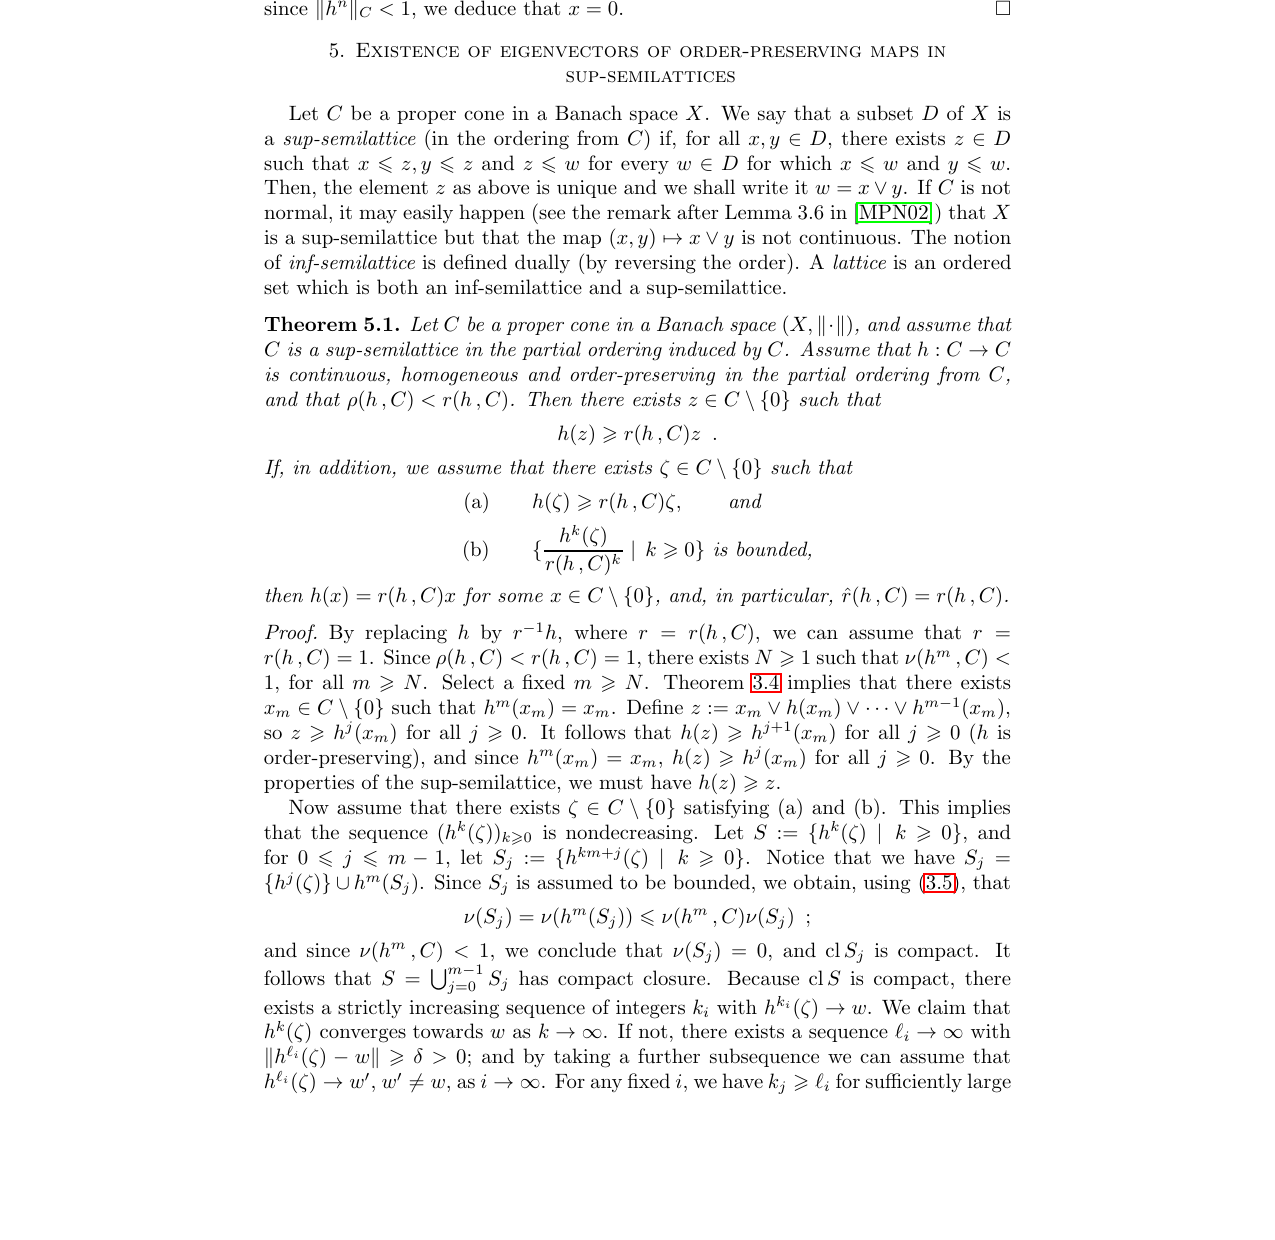
\includegraphics[width=0.96\linewidth]{figures/open_problem_context_page10.png}
\end{center}

\clearpage
\begin{center}
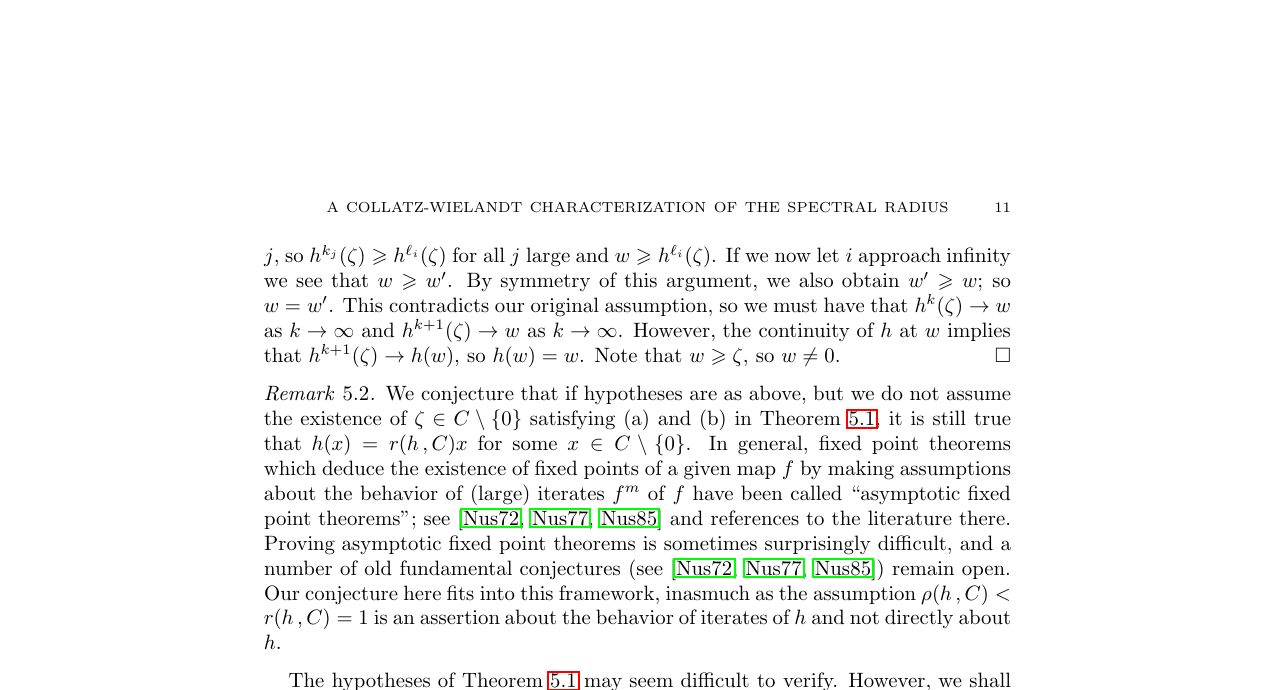
\includegraphics[width=0.96\linewidth]{figures/open_problem_conjecture_page11.png}
\end{center}

\noindent\textbf{Transcription of Remark 5.2.}
Under the preceding hypotheses, but without the extra vector satisfying
conditions (a) and (b) of Theorem 5.1, the authors conjecture that there is
still \(x\in C\setminus\{0\}\) such that
\(h(x)=r(h,C)x\) \cite[Remark 5.2]{AGN}.

\section{Definitions and proof intuition}

For a positively homogeneous self-map \(h\) of \(C\), the source defines

\[
 r(h,C)=\sup_{u\in C}\limsup_{n\to\infty}\|h^n(u)\|^{1/n}.
\]

Let \(\nu\) be the homogeneous generalized measure of noncompactness used in
the source. We use three of its stated properties:

\begin{enumerate}
\item \(\nu(A)=0\) if and only if \(\cl A\) is compact;
\item \(A\subseteq B\) implies \(\nu(A)\le\nu(B)\);
\item adjoining or deleting a relatively compact set, in particular finitely
many points, does not change \(\nu\) \cite[Proposition 3.3]{AGN}.
\end{enumerate}

The coefficient \(\nu(g,C)\) is defined so that

\[
  \nu(g(A))\le \nu(g,C)\nu(A)
\]

for every bounded \(A\subseteq C\). The definition of the essential spectral
radius implies that \(\essrad(h,C)<1\) yields an \(m\ge1\) with
\(\nu(h^m,C)<1\).

\paragraph{Proof intuition.}
The source already supplies a super-eigenvector \(z\le h(z)\). Its orbit can
be unbounded, but at spectral radius one it grows only subexponentially. Take
the running maximum \(A_n=\max_{j\le n}\|h^j(z)\|\). Subexponential growth
forces arbitrarily long almost-flat windows of \(A_n\). Choosing the left
endpoint at a genuine orbit-norm record gives unit vectors \(x_i\).

To recover compactness without assuming a bounded original orbit, look
backward from each record time. Every fixed backward shift remains in the
unit ball because the denominator is the later record maximum. Applying a
strictly condensing iterate \(h^m\) shifts one backward-record set onto the
preceding one, modulo a single point. Iterating the measure-of-noncompactness
inequality from arbitrarily far backward forces the record-vector set to
have measure zero. The almost-flat forward window then shows that a limit of
the record vectors has a bounded forward orbit.

\section{Two lemmas}

\begin{lemma}[Flat record times]\label{lem:records}
Let \((A_n)_{n\ge0}\) be a positive, nondecreasing, unbounded sequence with

\[
  \lim_{n\to\infty} A_n^{1/n}=1.
\]

Suppose \(A_n=\max_{0\le j\le n}a_j\) for a positive sequence \((a_j)\).
For every fixed positive integer \(m\), there are strictly increasing
integers \(k_i>im\) such that

\[
  a_{k_i}=A_{k_i},
  \qquad
  1\le \frac{A_{k_i+i}}{A_{k_i}}<e^{1/i}.
  \tag{1}
\]
\end{lemma}

\begin{proof}
For every positive integer \(L\) and every \(\eta>0\), there are arbitrarily
large \(n\) such that

\[
  A_{n+L}<e^\eta A_n. \tag{2}
\]

Indeed, if the reverse inequality held for all sufficiently large \(n\),
iteration along one arithmetic progression of step \(L\) would give

\[
  \liminf_{n\to\infty}A_n^{1/n}\ge e^{\eta/L}>1,
\]

a contradiction.

Inductively take \(n_i\) satisfying (2) with \(L=i\) and
\(\eta=1/i\), so large that \(A_{n_i}\) exceeds every \(a_j\) with
\(j\le\max\{im,k_{i-1}\}\). Choose \(k_i\le n_i\) with
\(a_{k_i}=A_{n_i}\). Then \(k_i>\max\{im,k_{i-1}\}\), and
\(A_{k_i}=A_{n_i}\). If \(k_i+i\le n_i\), monotonicity gives
\(A_{k_i+i}=A_{k_i}\). Otherwise \(k_i+i\le n_i+i\), so

\[
 \frac{A_{k_i+i}}{A_{k_i}}
 \le \frac{A_{n_i+i}}{A_{n_i}}<e^{1/i}.
\]

This proves (1).
\end{proof}

\begin{lemma}[Compactness from backward records]\label{lem:compact}
Let \(z_n=h^n(z)\), let \(A_n=\max_{0\le j\le n}\|z_j\|\), and suppose
the indices \(k_i\) satisfy Lemma \ref{lem:records} with
\(a_j=\|z_j\|\). If \(c:=\nu(h^m,C)<1\), then

\[
  \left\{\frac{z_{k_i}}{A_{k_i}}:i\ge1\right\}
\]

has compact closure.
\end{lemma}

\begin{proof}
For every integer \(q\ge0\), set

\[
 E_q=
 \left\{
   \frac{z_{k_i-qm}}{A_{k_i}}:i\ge q+1
 \right\}.
\]

The indices are nonnegative because \(k_i>im\). Also \(E_q\) is contained
in the closed unit ball \(B_X\): for \(i\ge q+1\),

\[
 \left\|\frac{z_{k_i-qm}}{A_{k_i}}\right\|
 \le \frac{A_{k_i}}{A_{k_i}}=1.
\]

Positive homogeneity gives

\[
 E_q=h^m(E_{q+1})\cup
 \left\{\frac{z_{k_{q+1}-qm}}{A_{k_{q+1}}}\right\}.
\]

Finite-set invariance of \(\nu\) and the definition of \(c\) imply

\[
  \nu(E_q)=\nu(h^m(E_{q+1}))\le c\nu(E_{q+1}).
\]

Since every \(E_q\subseteq B_X\), iteration yields, for every \(N\ge1\),

\[
  \nu(E_0)\le c^N\nu(E_N)\le c^N\nu(B_X).
\]

The number \(\nu(B_X)\) is finite and \(c<1\), hence \(\nu(E_0)=0\).
The defining compactness property of \(\nu\) completes the proof.
\end{proof}

\section{Full solution}

\begin{theorem}\label{thm:main}
Let \(C\) be a proper cone in a Banach space \(X\), and assume that \(C\) is
a sup-semilattice in its induced order. Let \(h:C\to C\) be continuous,
positively homogeneous, and order-preserving. If

\[
  \essrad(h,C)<r(h,C),
\]

then there is \(y\in C\setminus\{0\}\) such that

\[
  h(y)=r(h,C)y.
\]

Thus the conjecture in Remark 5.2 of \cite{AGN} holds in full.
\end{theorem}

\begin{proof}
Put \(r=r(h,C)\). The strict spectral gap implies \(r>0\). Replacing \(h\)
by \(r^{-1}h\), we may assume

\[
  r(h,C)=1,
  \qquad
  \essrad(h,C)<1. \tag{3}
\]

The first conclusion of Theorem 5.1 in \cite{AGN} gives
\(z\in C\setminus\{0\}\) such that \(z\le h(z)\). Let

\[
  z_n=h^n(z),
  \qquad
  A_n=\max_{0\le j\le n}\|z_j\|.
\]

The sequence \((z_n)\) is increasing in the cone order. By the definition of
the cone spectral radius and (3),

\[
  \limsup_{n\to\infty}\|z_n\|^{1/n}\le1.
\]

It follows that

\[
  \lim_{n\to\infty}A_n^{1/n}=1. \tag{4}
\]

For completeness, the upper bound follows because, for every
\(\varepsilon>0\), all sufficiently late \(z_j\) satisfy
\(\|z_j\|\le(1+\varepsilon)^j\), while the finitely many earlier norms are
absorbed by a constant. The lower bound follows from
\(A_n\ge\|z\|>0\).

If \((A_n)\) is bounded, then the orbit \((h^n(z))\) is bounded. Conditions
(a) and (b) of Theorem 5.1 are satisfied by \(z\), and that theorem gives a
nonzero fixed point of \(h\). Assume from now on that \((A_n)\) is unbounded.

By (3), choose \(m\ge1\) such that

\[
  c:=\nu(h^m,C)<1. \tag{5}
\]

Apply Lemma \ref{lem:records} to \(a_j=\|z_j\|\), and set

\[
  x_i=\frac{z_{k_i}}{A_{k_i}}.
\]

Since \(\|z_{k_i}\|=A_{k_i}\), every \(x_i\) has norm one. Lemma
\ref{lem:compact} shows that \((x_i)\) has a norm-convergent subsequence.
Relabel it so that \(x_i\to x\). Then \(x\in C\) and \(\|x\|=1\).

Since \(z_{k_i}\le z_{k_i+1}\), we have \(x_i\le h(x_i)\). The cone is
closed and \(h\) is continuous, so

\[
  x\le h(x). \tag{6}
\]

It remains to show that the forward orbit of \(x\) is bounded. Fix
\(j\ge0\). For all sufficiently large \(i\ge j\), (1) gives

\[
 \|h^j(x_i)\|
 =\frac{\|z_{k_i+j}\|}{A_{k_i}}
 \le\frac{A_{k_i+i}}{A_{k_i}}
 <e^{1/i}.
\]

Continuity of the fixed iterate \(h^j\) and \(x_i\to x\) therefore imply

\[
  \|h^j(x)\|\le1 \qquad(j\ge0). \tag{7}
\]

Thus \(x\ne0\), (6) is the super-eigenvector condition, and (7) is the
bounded-orbit condition in the second part of Theorem 5.1. That theorem now
provides \(y\in C\setminus\{0\}\) with \(h(y)=y\). Undoing the normalization
gives \(h(y)=r(h,C)y\).
\end{proof}

\section{Verification, scope, and novelty boundary}

The proof uses neither normality of the cone nor norm monotonicity. The
running maximum \(A_n\), rather than \(\|z_n\|\) itself, is what makes all
backward record shifts uniformly bounded. It also uses no uniform continuity
on bounded sets: only continuity of each fixed iterate is needed after the
compact subsequence is obtained.

The local result ledger, solution and attempt indexes, proof-gap index, and
full parsed arXiv source corpus were searched for arXiv:1112.5968 and the
phrases ``Remark 5.2'', ``asymptotic fixed point'', ``bounded orbit'',
``record time'', and ``cone essential spectral radius''. An external exact-
phrase search and the 30-work OpenAlex citation set for the source were also
checked, including the nearby works arXiv:1302.3905, arXiv:1406.6657,
arXiv:1612.01755, and the 2017 paper of Thieme on order-bounded maps. No later
statement resolving Remark 5.2, and no matching record-time proof, was found.
This was a bounded search rather than a systematic review, so novelty remains
subject to expert literature review.

\section{Human review focus}

Review is recommended in the following order:

\begin{enumerate}
\item verify the arbitrarily late flat-window assertion (2);
\item verify that choosing an actual record index preserves the flat window;
\item check the identity expressing \(E_q\) as \(h^m(E_{q+1})\) with one
indexed point adjoined;
\item check that all \(E_q\) lie in the same unit ball, uniformly in \(q\);
\item verify the fixed-\(j\) limiting argument that yields the bounded orbit
in (7).
\end{enumerate}

\begin{thebibliography}{9}

\bibitem{AGN}
M. Akian, S. Gaubert, and R. Nussbaum,
\emph{A Collatz--Wielandt characterization of the spectral radius of
order-preserving homogeneous maps on cones},
arXiv:1112.5968.
\url{https://arxiv.org/abs/1112.5968}

\end{thebibliography}

\end{document}
